\section{MVP}

\textbf{MVP} gehört zu den \textbf{MV*-Architekturmustern}.\\

\noindent
\textbf{Architekturmuster} besitzen wie \textbf{Entwurfsmuster} einen hohen Abstraktionsgrad.\\

\textbf{Entwurfsmuster} werden i.d.R. zur Lösung kleiner Teilbereiche von Software eingesetzt, während \code{Arhictekturmuster} für die gesamte Software oder für größere Teile einer Software eingesetzt werden\footnote{vgl. Skript FOPT4, S. 1}.\\
$\rightarrow$ Entwurfsmuster beschreiben eher das Zusammenwirken von Klassen und Schnittstellen.
Architekturmuster sind wie ein Bauplan für ganze Programmteile bzw. Teilbereiche einer Software zu verstehen.

\noindent
zu den Vorteilen von Architekturmustern gehört:

\begin{itemize}
    \item sie helfen, Anwendungen klarer zu strukturieren $\rightarrow$ Leitfaden zur Strukturierung
    \item erleichtert das systematische Testen (durch klare Strukturierung); Änderungen an der Software sind leichter durchführbar
    \item hilft, den Code anderer zu verstehen, wenn dieser nach einem bestimmten Muster strukturiert ist
\end{itemize}

\subsection{Prinzip von MVP}

\textbf{MVP} bezeichnet drei Komponenten: \textbf{Model}, \textbf{View}, \textbf{Presenter}.\\

\subsection*{Model}

Das \textbf{Model} ist verantwortlich für
\begin{itemize}
    \item die \textbf{Geschäftslogik}, die den logischen Kern der Anwendung darstellt
    \item die Bereitstellung und das Ändern relevanter Daten für die Anwendung
    \item die Wahrung von Konsistenzbedingungen
    \item die Realisierung von Persistierung
\end{itemize}

Das Model ist unabhängig von Darstellungs- und Steuerungslogik.

\subsection*{View}

Die \textbf{View} ist die Darstellungskomponente der Software und baut und verändert sie.\\
Mehrere Views können hierbei Teile des Models darstellen.\\
Benutzerinteraktionen werden von der View an den Presenter weitergeleitet.\\

\subsection*{Presenter}
Die \textbf{Präsentationskomponente} ist zuständig für die Ablaufsteuerung, i.d.R. durch vom Bentzer ausgelöste Aktionen, wie bspw. einem Button-click.

\begin{tcolorbox}
Der \textbf{Presenter} hat eine Vermittlerrolle: Er kennt das \textbf{Model} und kann bei Bedarf vermitteln.\\
Im Unterschied zu \textbf{MVC} kennen sich Model und \textbf{View} nicht (s. Abbildung~\ref{fig:mvp}).\\
\end{tcolorbox}

\begin{figure}
    \centering
    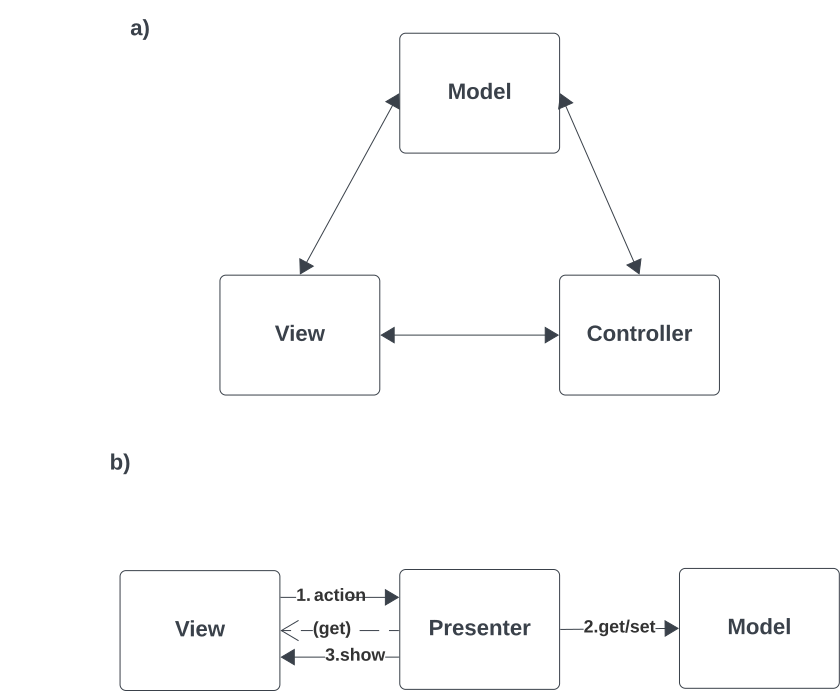
\includegraphics[scale=0.5]{chapters/fopt4/img/mvp}
    \caption{Während bei MVC die Komponenten direkt  Informationen untereinander austauschen können, kennen sich bei MVP Model und View nicht, vermittelt wird über den Presenter. Der Presenter ist auch in der Lage, sich Daten von der View zu beschaffen. (Quelle: in Anlehnung an \cite[223, Bild 4.12]{Oec22})}
    \label{fig:mvp}
\end{figure}


\noindent
Der Presenter kann einen Teil der Validierungslogik enthalten, bspw. zum Erkennen fehlerhafter Eingabedaten.\\

\noindent
Alle Komponenten sind gut testbar:

\begin{itemize}
    \item Das \textbf{Model} hat keine Abhängigkeiten zu \textbf{Presenter} und \textbf{View}.
    \item Der \textbf{Presenter} kann über \textit{Mock-Objekte} (für View & Models) getestet werden
    \item Die \textbf{View} erhält für den Presenter ein Mock-Objekt.
\end{itemize}

\section{Threads und JavaFX}

Stage-Objekte dürfen nicht im \textbf{Main-Thread} erzeugt werden. \\
Das primäre Stage-Objekt wird von der Platform vorgegeben, nachfolgenden Stage-Objekte und UI -Elemente müssen im \textbf{JavaFX Application Thread} erzeugt werden.\\

\noindent
Der \textbf{JavaFX Application Thread} ist auch zuständig für die Ereignisbehandlung - insgesamt gibt es nur einen solchen Thread für die Verwaltung von UI-Elementen und deren Ereignisse. \\

\noindent
Mit der Methode \staticcode{javafx.application.Platform.runLater()}) lassen sich Aktionen am \textbf{JavaFX Application Thread} \textit{anmelden} bzw. in dessen \textit{Warteschlange} einreihen (Parameter vom Typ \code{Runnable}).\\

\subsection*{Regel 1}
Die Durchführung der Ereignisbehandlung sollte in \ul{möglichst kurzer Zeit} abgeschlossen sein, auf \code{sleep()} und \code{wait()} sollte möglichst verzichtet werden.

\subsection*{Regel 2}
Der Zugriff auf grafische Elemente der Oberfläche darf \ul{ausschließlich} durch den \textbf{JavaFX Application Thread} erfolgen.\\
Wenn ein anderer Thread auf die Oberfläche zugreifen möchte, beauftragt der dazu den \textbf{JavaFX Application Thread} durch den Aufruf der Methode \code{Platform.runLater()}.\\
Der Auftrag muss in Form eines \code{Runnable}-Objektes übergeben werden.\\

\noindent
Um Theads, die mit der UI interagieren, mit Beendigung des Hauptprogramms zu beenden, sollte man sie als Daemon-Thread deklarieren\footnote{
``Ein Java-Programm ist zu Ende, wenn alle Threads zu Ende sind - Hintergrund-Threads werden dabei nciht beachtet, nur Vordergrund-Threads (vgl.~\cite[89]{Oec22}).
} (Aufruf der methode \code{setDaemon(true)} auf ein Objekt der Klasse \code{java.lang.Thread}, bevor der Thread gestartet wurde).\\

\noindent
\code{Runnable}s werden in der Reihenfolge durchgeführt, in denen sie mit \code{Platform.runLater()} angemeldet worden sind.

\subsection{Tasks und Services in JavaFX}

JavaFX bietet eine Unterstützung zur Verarbeitung länger andauernder / immer wiederkehrender Aktivitäten im Zusammenhanf mit der UI an, über die generische Schnittstelle \code{Worker} sowie der generischen Klassen \code{Task}, \code{Service}, \code{ScheduledService}.\\

\noindent
\textbf{Task} ermöglicht eine einmalige Ausführung einer länger andauernden Aktivität.\\

\noindent
\texbf{Service} ermöglicht die wiederholte Aktivierung, indem immer wieder Task-Objekte erzeugt werden.\\

\noindent
\textbf{ScheduledService} ermöglicht die periodische ADurchführung von Aktivitäten.\\

\noindent
Properties ermöglichen die Kommunikation zwischen \textbf{Tasks}/\code{Services} und dem \textbf{JavaFX Application Thread}, über sie kommt man sogar ohne \code{Platform.runLater()} aus (der gleichzeitige Gebrauch wird aber nicht ausgeschlossen.)\\

\noindent
Die Methode der Listener, die an diese Properties angemeldet sind, werden immer vom \textbf{JavaFX Application Thread} ausgeführt.\\

\noindent
Beispiele für Properties der Klasse \code{Task}\footnote{
Class Task<V>: \url{https://docs.oracle.com/javase/8/javafx/api/javafx/concurrent/Task.html} - abgerufen 29.01.2024
}:

\begin{itemize}
    \item \code{message}: Meldungen von Threads aus dem \textbf{JavaFX Application Thread; die Threads können über \code{updateMessage()}} den Inhalt ändern
    \item \code{title:} wie \code{message} (analoge Funktion: \code{setTitle()})
    \item \code{value}: ähnlich \code{message} und \code{title} (Methode: \code{updateValue()}); der Typ ist \code{ReadOnlyObjectProperty<V>}, wobei \code{V} der generische Typ der Klasse \code{Task} ist.
    \item \code{workDone} / \code{totalWork}: Indikator zum Fortschritt (Relation geleistete Arbeit zur gesamten Arbeit).
    \code{updateProgress()} ermöglicht die Aktualisierung beider Werte auf einmal
    \item \code{progress}: nur lesender Zugriff, liefert immer $\frac{workDone}{totalWork}$, also den Quotienten
    \item \code{state}: liefert den zustand des Tasks (\code{READY}, \code{RUNNING}, \code{SUCCEEDED}, \code{FAILED}, \code{CANCELLED})
\end{itemize}

Um \code{Task} zu verwenden, leitet man eine eigene Klasse von \code{Task} ab und überschreibt \code{call}; in der Methode lässt sich \code{updateValue} und \code{updateProgress} aufrufen (der Rückgabetyp von \code{call} its der Typparameter der KLasse \code{Task}; für \code{extends Task<Double>} also \code{Doubel}).\\
\code{call} sollte überprüfen, ob \code{cancel} aufgerufen wurde (\code{isCancelled}), um die Bearbeitung abzubrechen (im Gegensatz zum \code{interrupt}-Flag bei Threads ist der Zustand des \clode{cancel}-Flags aber persistent).\\

\noindent
\code{Service}s sind für wiederholte Ausführungen länger andauernde Aktivitäten vorgesehen: Services erzeugen hierfür bei jeder wiederholten Ausführung ein neues \code{Task}-Objekt; ein Service kann mittels \code{start()} direkt gestartet werden, ein \code{Task} implementiert die \code{Runnable}-Schnittstelle und wird einem Thread übergeben, der gestartet werden muss.

\begin{minted}[mathescape,
    linenos,
    numbersep=5pt,
    gobble=2,
    frame=lines,
    framesep=2mm]{java}
    MyTask t = new MyTask();
    Thread t1 = new Thread(t);
    t1.setDaemon(true);
    t1.start();
\end{minted}\\

\noindent
Eine Klasse muss von der abstrakten Klasse \code{Service} ableiten und darin \code{createTask()} überschreiben, die das entsprechende Task-Objekt zurückliefert.\\

\noindent
Man kann dem Service einen \code{Executor} zuweisen, ansonsten wird ein neuer \code{Daemon}-Thread erzeugt und gestartet.\\

\noindent
Erneutes Starten des Service ist erst möglich, wenn der Service nicht mehr aktiv ist (\code{isRunning}), oder wenn zuvor \code{reset()} aufgerufen wurde.\\
Auch \code{restart()} ermöglicht einen Neustart (ruft intern \code{cancel()} $\rightarrow$ \code{reset()} $\rightarrow$ \code{start()} auf).